\chapter{Testing and Evaluation}
\label{cha:testing}

\begin{comment}
Chapter 6: Testing and Evaluation
This chapter should give details of how the system designed and implemented by you was tested. The data and results obtained from this testing whould be presented and consideration be given as to whether or not these results confirm that everything works correctly.

The analysis of test results is very important and some assessment of their significance and quality must be given. Likely sources of error and inaccuracy should be mentioned. Use graphs, bar charts and histograms where appropriate, remembering to label all axes and give scales. The analysis is often done badly, thus sacrificing marks.
\end{comment}

The evaluation of the application indicates that these three objectives have been met. Preliminary research demonstrates that enjoyed using the application and that the majority of participants would use it in the future if implemented as a full product. Testing with participant data shows that the average absolute error of the prediction engine was $PERCENTAGE\%$ for users with over three months historical information. Preliminary penetration testing, using both white-box and black-box testing indicated that the security protections put in place are effective.  However, the evaluation of the project was limited, due to the size of the user base, discussed further in \autoref{sec:limitations}. \todo{Complete this}

\section{During Development}
Though-out the development of the project, predominantly after each feature was implemented and before a new iteration was started the applications functionality was tested through face to face conversations, observations and unit testing.

\subsection{Acceptance Testing}
As noted throughout the report, the application was regularly tested by potential end users and the developers during lab observations where the user was asked to complete a task on the website while describing what they were doing. 

During the testing, common pain points were identified and these were used to decide on the future features, either to improve the user experience on the website, making it easier to use, or to support a new use case.

Example modifications, made as a result of these observations, include the dropdown menu autocompletion when creating and mapping transactors, the hints that appear throughout the website to guide the user onto the next task, and the suggestion wizard.

Towards the beginning of the project these meetings were used to evaluate and update the design of the user interface, which went through several different designs, and to receive qualitative feedback from the users (Fig. \ref{fig:ui-design}).

\begin{figure}
\centering
\begin{subfigure}{0.34\textwidth}
  \centering
  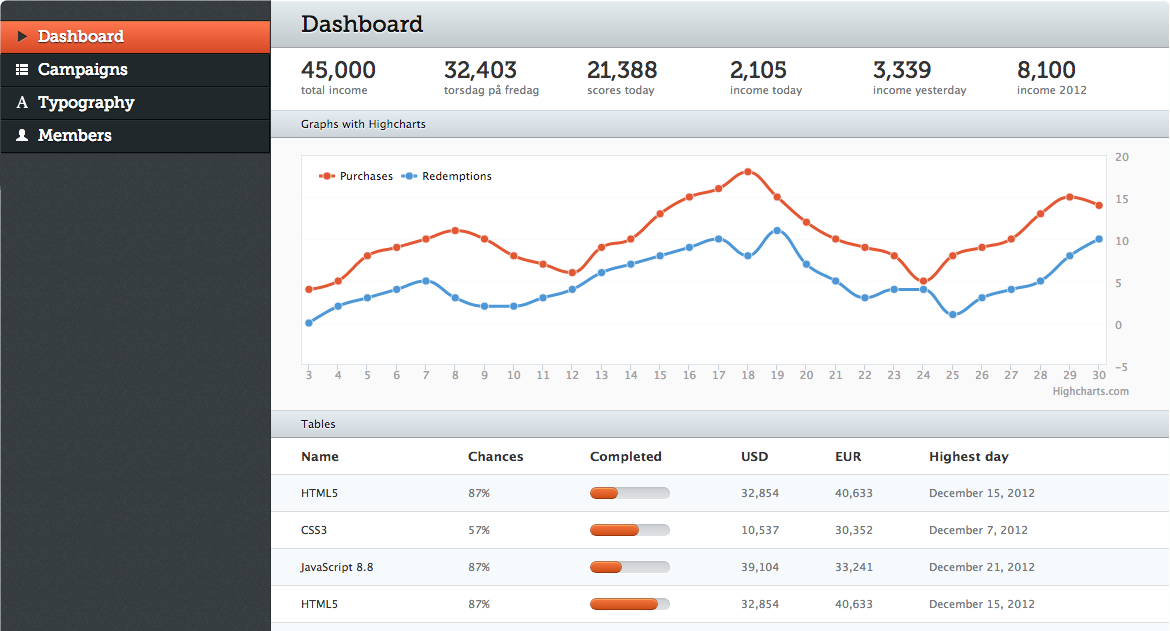
\includegraphics[width=0.95\linewidth]{testing/uidesign1}
\end{subfigure}%
\begin{subfigure}{0.34\textwidth}
  \centering
  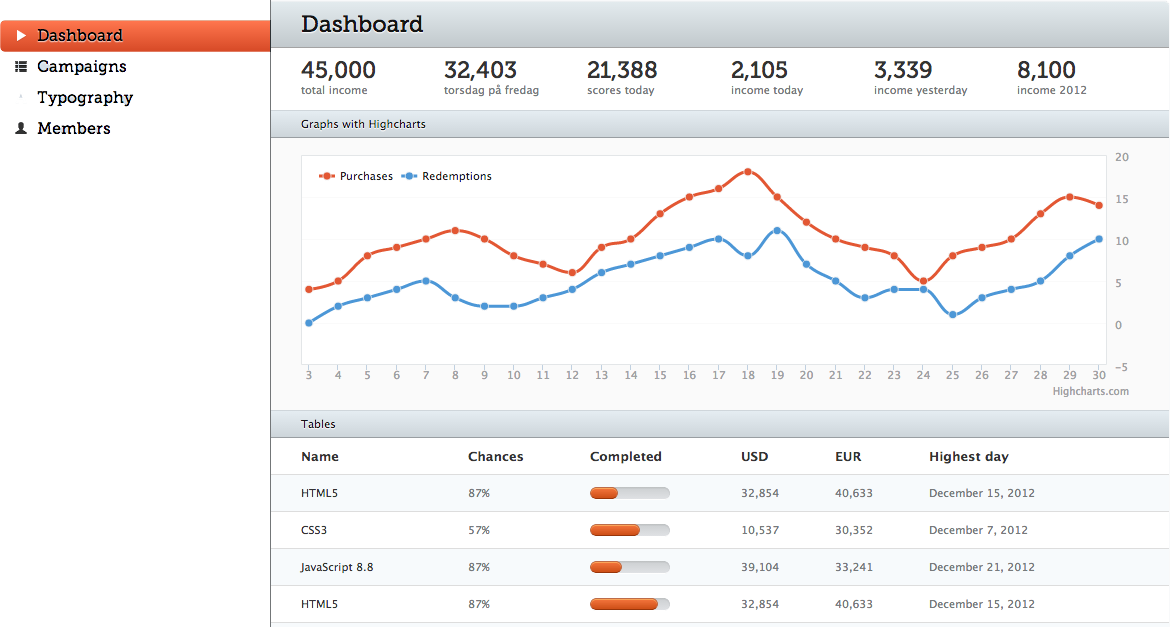
\includegraphics[width=0.95\linewidth]{testing/uidesign2}
\end{subfigure}
\begin{subfigure}{0.31\textwidth}
  \centering
  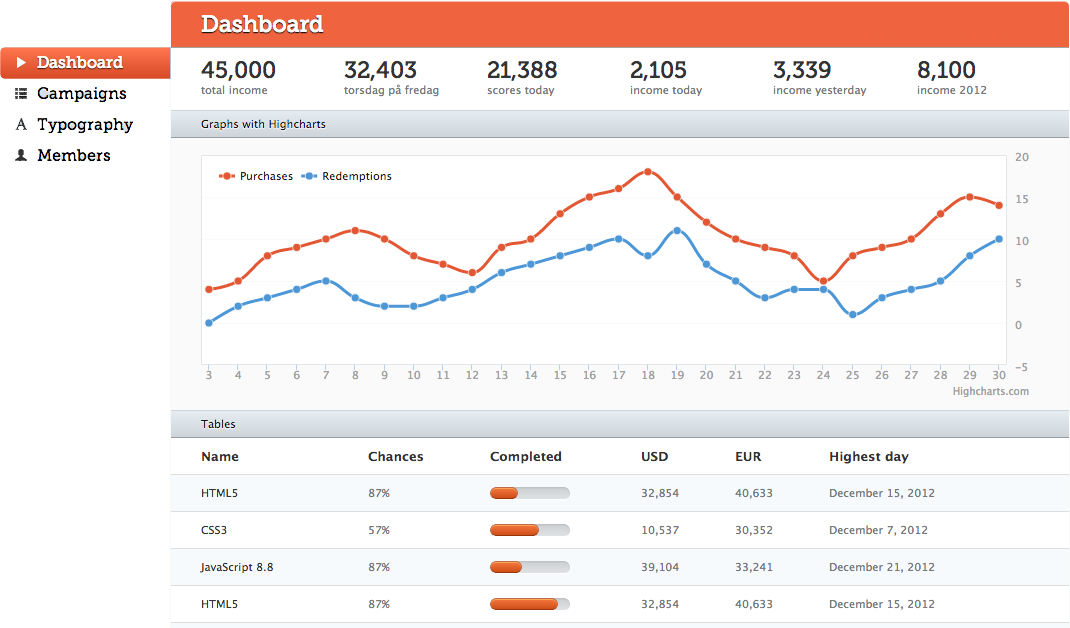
\includegraphics[width=0.95\linewidth]{testing/uidesign3}
\end{subfigure}
\caption{A few iterations of the user interface designs}
\label{fig:ui-design}
\end{figure}

\subsection{Unit Testing}
High risk classes, including the Budget, the QIF and OFX Parsers implementing the TransactionFileParserInterface, and those implementing the TransactionCollectionInterface were unit tested to ensure the functionality of the classes was not affected when implementing new features or refactoring the code.

These classes were selected as the core functionality of the application relied on their behaviour and they were coupled to the most other classes, for example the Budget object was responsible for holding a collection of Transactons in the tree data structure described in \autoref{section:prediction-implementation} and performed the majority of the prediction functionality, holding references to the TransactionMarkovChain, TransactionWeightedAverageCalculator and PredictionEvaluation.

Due to time constraints and the complications of testing data driven classes, both the number of unit tested classes and methods covered was limited, this is discussed further in \autoref{sec:limitations}.

\section{After Development}
Once development of the project was halted the application was tested in the three following the three sections outlined through the report. The statement management functionality was assessed using a questionnaire posed to research participants that were given access to the system, the prediction algorithms were evaluated using the sample data provided by the research participants and the security of the application was evaluated using penetration testing.
%
Unfortunately the reliability of the results for both the statement management and prediction is questionable due to the limited number of research participants and questionnaire responses, see \autoref{sec:limitations}.

% This chapter should give details of how the system designed and implemented by you was tested. The data and results obtained from this testing whould be presented and consideration be given as to whether or not these results confirm that everything works correctly.
% The analysis of test results is very important and some assessment of their significance and quality must be given. Likely sources of error and inaccuracy should be mentioned. Use graphs, bar charts and histograms where appropriate, remembering to label all axes and give scales. The analysis is often done badly, thus sacrificing marks.

\subsection{Statement Management}
The questionnaire posed to the research participants was split into three sections, a full copy of the questions can be found in Appendix \ref{app:questionnaire}.

The first made a series of statements and asked the respondent to answer on a five point scale, ranging from 1, strongly disagree to 5, strongly agree. The questions in this sections had four main types, and were selected following the structure of the Standardized Universal Percentile Rank-Questionnaire \ref{sauro2011standardized} which is used by companies including PayPal to assess their websites. 
%
Questions on usability focused on how easy users found navigation of the website, locating the information they needed, and whether they enjoyed using it.
%
Credibility questions focused on whether the user trusted the website having uploaded their personal information.
%
The likely hood of a user recommending the site to their colleagues and friends or returning to the site in the future gave an idea of the potential loyalty the participants expressed.
%
The last focused on the user interface to gain an idea of whether the website appealed to the users.

The second section focused on task completion, participants were asked to complete a task and then rate the how difficult or easy they found that on a seven point scale.
%
This section was designed to assess the functionality of the website and to identify additional pain points.
%
One scale question was asked per task as research suggests that use of a single question performs just as well as breaking the task down into sub-questions \parencite{sauro2009comparison, sauro2009correlations}, however a free text field was included with each task to obtain qualitative information on the reasons behind the answer.

In final section was used to identify features of the the website that users favoured and to allow for feature requests, all questions were answered in free text fields

The average respondant said the website was easy to nativate, 3.80.

Comfortable using the website: 3.80

Completed visit 4.20
Reccoment website if complete 4.00

Attractive 3.80

Downloading from bank 5.40
Upload statement 6.80
View statement 6.00
Prediction 4.40
Overall use: 5.60

\subsection{Prediction}

\subsection{Security}

% The evaluation of the application indicates that these three objectives have been met. Preliminary research demonstrates that enjoyed using the application and that the majority of participants would use it in the future if implemented as a full product. Testing with participant data shows that the average absolute error of the prediction engine was $PERCENTAGE\%$ for users with over three months historical information. Preliminary penetration testing, using both white-box and black-box testing indicated that the security protections put in place are effective.  However, the evaluation of the project was limited, due to the size of the user base, discussed further in \autoref{sec:limitations}. \todo{Complete this}

\plan{How did I check that it was working? Testing with personal data, users trying it and running tests of everything}

\missingfigure{Need figures representing accuracy, error, etc}

\section{User feedback}

% SUPR-Q - http://www.measuringusability.com/suprq.php


\plan{User surveys to check what they wanted}
